\documentclass{beamer}
\usepackage{amsmath}
\usepackage{amssymb}
\usepackage{pgf}
\usepackage{tikz}
\usepackage{listings}
\usepackage{color}
\usetikzlibrary{matrix}
\usetheme{boxes}
\newcommand{\fig}{figures} % common figure path
\newcommand{\dbbslsh}{\textbackslash \textbackslash} % common figure path
\newcommand{\frnzplt}{FranzPlot }
\newenvironment{myblock}[3]{%
\definecolor{smtbx}{rgb}{0.64,0.76,0.68}
\setbeamercolor{block body}{#2}
\setbeamercolor{block title}{#3}
\begin{block}{#1}}{\end{block}}
\title[Curve e Sup. - Lab 5]{Curve e Superfici per il Design \\ Laboratorio 5 - Curve parametriche}
\author[Prof.ssa Scotti]{Prof. Nicola Parolini}
%\institute[dimat]{Long Inst.}
\date{21 Novembre 2019}

\begin{document}
%\lstset{language=POV}
\begin{frame}
\maketitle
\end{frame}
\section{Introduzione}
\begin{frame}
\frametitle{Materiali}
Nella cartella con il materiale di oggi troverete:
\begin{itemize}
\item Questa presentazione \\ (\texttt{Materiale Didattico/Laboratori/lab 5/lab5\_testo.pdf});
%\item Il file \texttt{es\_dado\_ref.toml} con l'esercizio risolto della passata esercitazione.
\item L'eseguibile del \frnzplt \\ (\texttt{Software/Franzplot 19.08 - Windows.exe})
\end{itemize}
\end{frame}

\section{Riepilogo}
%
\begin{frame}
\frametitle{Esercizio 1: Curve con \frnzplt - Il comando parametric curve}
Sia data la seguente curva:
\begin{displaymath}
c:
\begin{cases}
    x = cos(t)\\
    y = 2 sin(t)\\
    z = 0.5
\end{cases}
\end{displaymath}
    con $t \in [0, 2\pi]$. \\
Vogliamo rappresentarla con \frnzplt attraverso l'elemento `parametric curve'.
\end{frame}
%

\begin{frame}
\frametitle{Esercizio 1 - i}
    Come avevamo visto nel caso del plot di rette, anche oggi faremo uso dei seguenti nodi:
    \begin{itemize}
        \item \texttt{Geometries > Curve} 
        \item \texttt{Parameters > Interval}
        \item \texttt{Geometry Renderer}
    \end{itemize}

    \vspace{0.5cm}
    A differenza della visualizzazione di una retta, questa volta sar\`a fondamentale assegnare i valori corretti
    all'inizio e la fine dell'intervallo.
\end{frame}
%
\begin{frame}
\frametitle{Esercizio 1 - ii}
\begin{center}
\begin{tikzpicture}
\node(img1){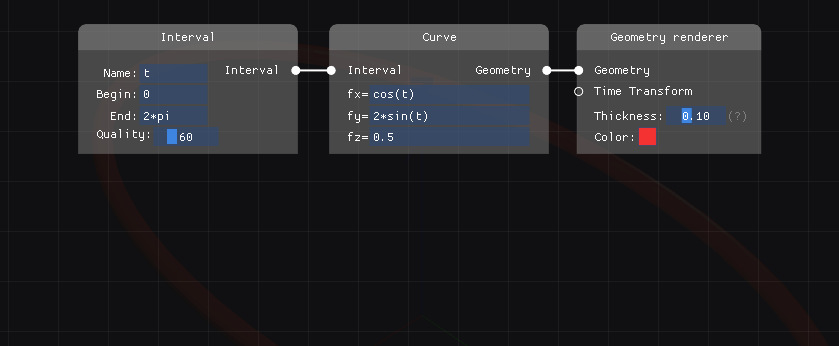
\includegraphics[width=0.8\textwidth]{\fig/lab5_es1_graph.png}};
\node(img2) at (img1.south){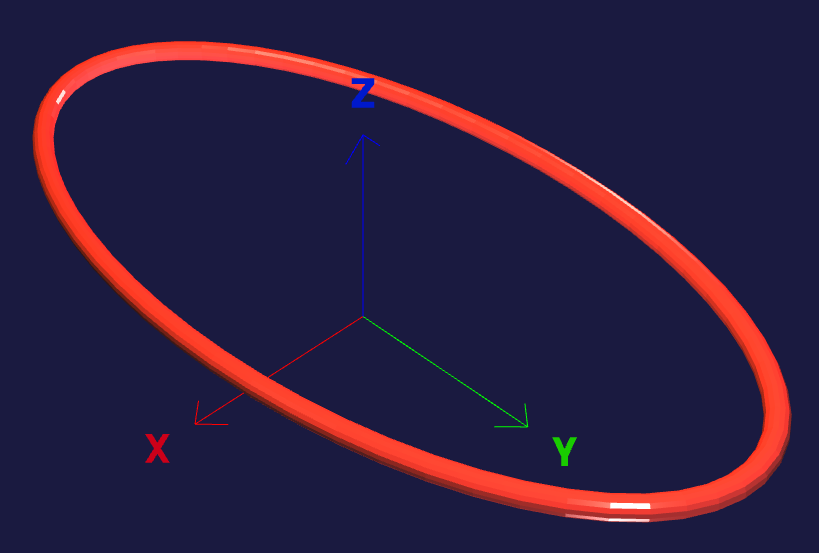
\includegraphics[width=0.5\textwidth]{\fig/lab5_es1_scene.png}};
\end{tikzpicture}
\end{center}
    Il parametro ``quality'' indica quanti punti saranno usati dal \frnzplt per
    approssimare la curva (o la superficie)

\end{frame}
%%
\begin{frame}
\frametitle{Esercizio 2: Rotazione di un punto}

    Sia dato il punto $P(0, 1, 1)$.
    \begin{itemize}
        \item Scrivere la generica matrice $R$ di rotazione intorno l'asse Z.
        \item Applicare a $P$ una trasformazione parametrica di rotazione intorno l'asse Z, con parametro $\theta \in [0, \pi]$,
            e scrivere la curva parametrica ottenuta. Di che curva si tratta?
        \item Rappresentare il punto $P$ e la curva ottenuta in \frnzplt.
        \item Usando \frnzplt, disegnare la curva applicando al punto una matrice parametrica.
    \end{itemize}

\end{frame}

\begin{frame}
\frametitle{Esercizio 2 - i}
La matrice che rappresenta la trasformazione parametrica \`e la seguente:
\begin{equation}
R(\theta) = 
\begin{bmatrix}
    \mbox{cos}(\theta) & - \mbox{sin}(\theta) & 0 & 0\\
    \mbox{sin}(\theta) & \mbox{cos}(\theta)   & 0 & 0\\ 
    0 & 0 & 1 & 0 \\
    0 & 0 & 0 & 1
\end{bmatrix}
\quad
    \theta \in [0, \pi]
\end{equation}

    Per ottenere la curva dobbiamo moltiplicarla per il vettore che contiene le coordinate del punto: 
    $$
    c(\theta) = R(\theta) P
    $$
\end{frame}

\begin{frame}
\frametitle{Esercizio 2 - ii}
Svolgendo i conti troviamo:
\begin{equation}
c(\theta) = 
\begin{bmatrix}
    \mbox{cos}(\theta) & - \mbox{sin}(\theta) & 0 & 0\\
    \mbox{sin}(\theta) & \mbox{cos}(\theta)   & 0 & 0\\ 
    0 & 0 & 1 & 0 \\
    0 & 0 & 0 & 1
\end{bmatrix}
\cdot
\begin{bmatrix}
    0 \\
    1 \\
    1 \\
    1
\end{bmatrix}
 = 
\begin{bmatrix}
    -sin(\theta) \\
    cos(\theta) \\
    1 \\
    1
\end{bmatrix}
\end{equation}
Quindi possiamo scrivere la nostra curva:
\begin{displaymath}
    c(\theta):
\begin{cases}
    x = -sin(\theta) \\
    y = cos(\theta) \\
    z = 1 \\
\end{cases}
\quad
    \theta \in [0, \pi]
\end{displaymath}

Poich\'e $\theta$ varia da $0$ a $\pi$, la curva \`e una semicirconferenza.
\end{frame}

\begin{frame}
\frametitle{Esercizio 2 - iii}
\begin{center}
\begin{tikzpicture}
\node(img1){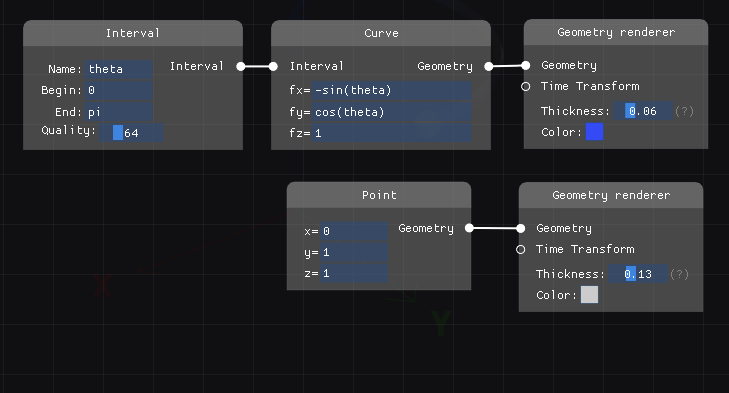
\includegraphics[width=0.8\textwidth]{\fig/lab5_es2_graph.png}};
\node(img2) at (img1.south west){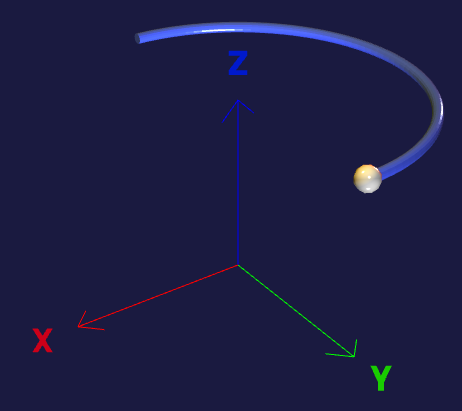
\includegraphics[width=0.4\textwidth]{\fig/lab5_es2_scene.png}};
\end{tikzpicture}
\end{center}

\end{frame}

\begin{frame}
\frametitle{Esercizio 2 - iv}
    Nel \frnzplt \`e possibile scrivere matrici parametriche e usare il nodo \texttt{Transform} per
    applicare una trasformazione parametrica a una geometria 0D o 1D (punto o curva).

    \begin{itemize}
        \item Nota: non \`e possibile applicare trasformazioni parametriche a primitive come cubi, dadi, ecc
    \end{itemize}

    \vspace{1cm}
    Per scrivere una trasformazione parametrica, \`e sufficiente usare il nodo
    \texttt{Generic Matrix}, collegare in input l'\texttt{Interval} del parametro da usare,
    e scrivere espressioni contenenti il parametro all'interno della matrice.

\end{frame}

\begin{frame}
\frametitle{Esercizio 2 - v}
\begin{center}
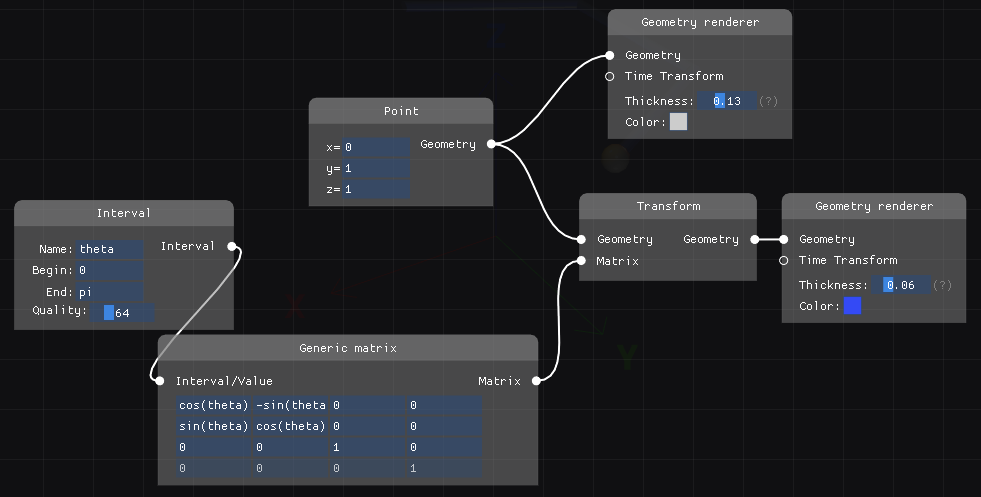
\includegraphics[width=\textwidth]{\fig/lab5_es2_param_transform.png}
\end{center}

    Come sempre il nome del parametro \`e arbitrario (\texttt{theta}, \texttt{t}, \texttt{r}, sono tutti validi).
    L'importante \'e essere \textbf{consistenti}.
\end{frame}
%
\begin{frame}
\frametitle{Esercizio 3: Spirale conica}
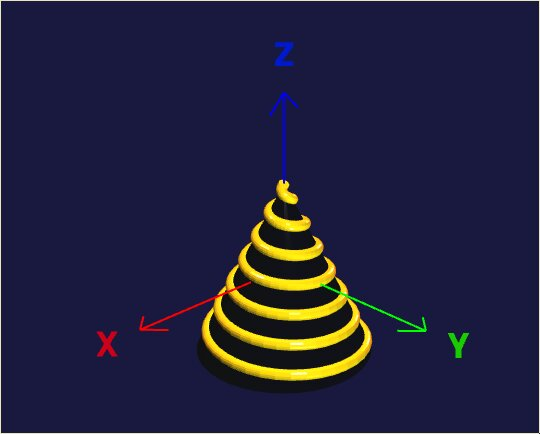
\includegraphics[width=0.5\textwidth]{\fig/cone_spiral.jpeg}\\
Determinare la curva parametrica che descrive il filo avvolto sul cono (da \texttt{primitive}). 
\end{frame}
\begin{frame}
\frametitle{Esercizio 3-ii}
La curva \`e data dalla rotazione di un punto intorno all'asse, con raggio
variabile, composta con una traslazione lungo lo stesso asse, quindi si tratta
di un'elica conica.  
\begin{displaymath}
\mathcal{C}:\begin{cases}
 x(t)= at\cos t\\
 y(t)=at \sin t\\
  z(t)= ct + d \qquad t_I\leq t\leq 0
\end{cases}
\end{displaymath}
Il rapporto fra $a$ e $c$ \`e legato alla semiapertura del cono. Usiamo valori
di $t$ negativi per disegnare il tratto inferiore dell'elica conica e $d$ per
traslare il vertice lungo $z$.  
\end{frame}
\begin{frame}
\frametitle{Esercizio 4: Sole/Terra/Luna}
L'equazione parametrica della circonferenza, ad esempio:
\begin{displaymath}
\mathcal{C}:\begin{cases}
 x(t)= a \cos t\\
 y(t)= a \sin t\\
 z(t)= 0
\end{cases}
\end{displaymath}
\`e utile anche per descrivere l'orbita dei corpi celesti. \\
Ponendo il sole al centro del sistema di riferimento, scrivere la curva che descrive il moto di un pianeta e di un suo satellite.\\
\begin{block}{Suggerimento}
Per ogni valore del parametro t, il moto del satellite rispetto al pianeta pu\`o essere visto come una rotazione
attorno al centro degli assi traslato della posizione del pianeta.  
\end{block}
\begin{itemize}
\item Rappresentare lo stesso sistema utilizzando punti e/o sfere ed il nodo \texttt{time transform}.
\end{itemize}
\end{frame}

\begin{frame}
\frametitle{Esercizio 4 - ii}

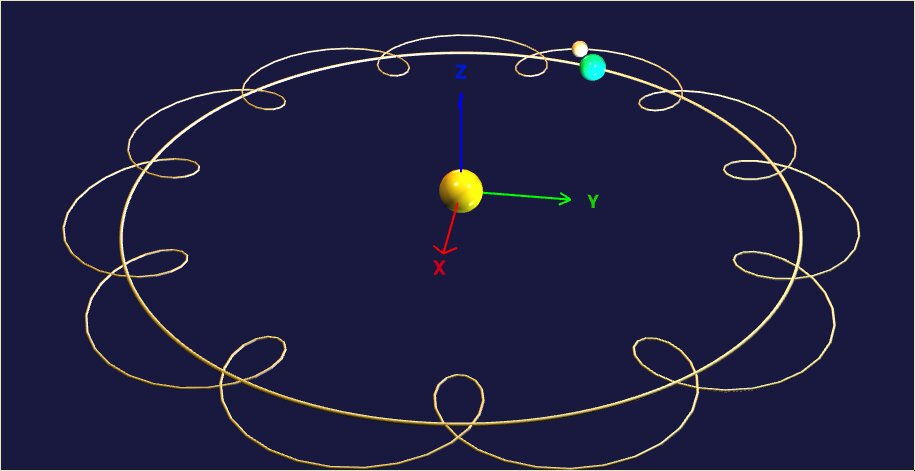
\includegraphics[width=0.8\textwidth]{\fig/sunsys.jpeg}
\\
Una curva come quella in figura \`e  qualitativamente l'unico tipo di curva osservabile?
\end{frame}


\begin{frame}
\frametitle{Esercizio 5}

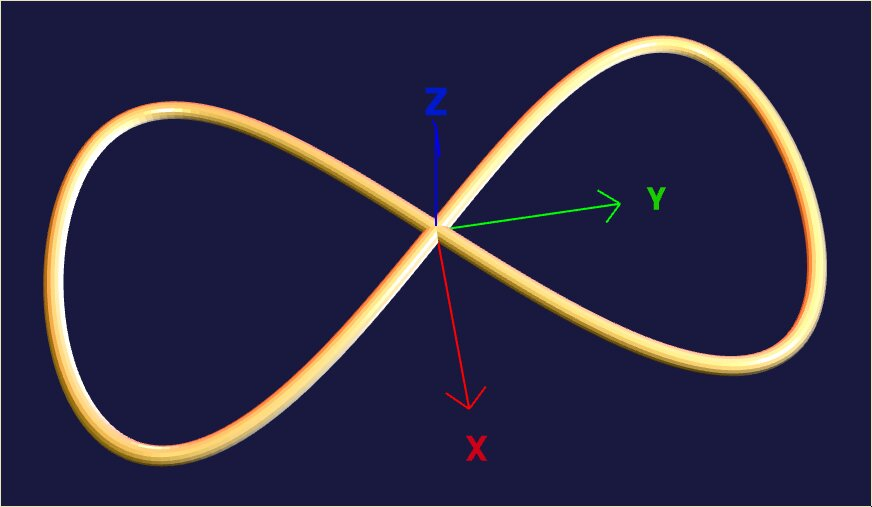
\includegraphics[width=0.8\textwidth]{\fig/infty.jpeg}

Determinare la forma della equazione parametrica che descrive questa curva. 
\end{frame}

\end{document}
